\documentclass[]{article}
\hyphenation{co-rres-pon-dien-tes te-ner E-ben-sper-ger de-pre-da-do-res dis-po-ni-ble be-ne-fi-cio-sa in-di-vi-dual so-cia-li-dad mos-tra-ron fuen-tes a-cep-ta-ble ta-ma-ño o-pues-ta mo-de-lo es-tu-dian-tes e-jer-ci-cios co-rres-pon-dien-te mo-di-fi-ca-dos mo-di-fi-car-lo ma-ni-pu-lar}
\usepackage{amssymb,amsmath}
\usepackage{ifxetex,ifluatex}
\ifxetex
  \usepackage{fontspec,xltxtra,xunicode}
  \defaultfontfeatures{Mapping=tex-text,Scale=MatchLowercase}
\else
  \ifluatex
    \usepackage{fontspec}
    \defaultfontfeatures{Mapping=tex-text,Scale=MatchLowercase}
  \else
    \usepackage[utf8]{inputenc}
  \fi
\fi
\usepackage{color}
\usepackage{fancyvrb}
\DefineShortVerb[commandchars=\\\{\}]{\|}
\DefineVerbatimEnvironment{Highlighting}{Verbatim}{commandchars=\\\{\}}
% Add ',fontsize=\small' for more characters per line
\newenvironment{Shaded}{}{}
\newcommand{\KeywordTok}[1]{\textcolor[rgb]{0.00,0.44,0.13}{\textbf{{#1}}}}
\newcommand{\DataTypeTok}[1]{\textcolor[rgb]{0.56,0.13,0.00}{{#1}}}
\newcommand{\DecValTok}[1]{\textcolor[rgb]{0.25,0.63,0.44}{{#1}}}
\newcommand{\BaseNTok}[1]{\textcolor[rgb]{0.25,0.63,0.44}{{#1}}}
\newcommand{\FloatTok}[1]{\textcolor[rgb]{0.25,0.63,0.44}{{#1}}}
\newcommand{\CharTok}[1]{\textcolor[rgb]{0.25,0.44,0.63}{{#1}}}
\newcommand{\StringTok}[1]{\textcolor[rgb]{0.25,0.44,0.63}{{#1}}}
\newcommand{\CommentTok}[1]{\textcolor[rgb]{0.38,0.63,0.69}{\textit{{#1}}}}
\newcommand{\OtherTok}[1]{\textcolor[rgb]{0.00,0.44,0.13}{{#1}}}
\newcommand{\AlertTok}[1]{\textcolor[rgb]{1.00,0.00,0.00}{\textbf{{#1}}}}
\newcommand{\FunctionTok}[1]{\textcolor[rgb]{0.02,0.16,0.49}{{#1}}}
\newcommand{\RegionMarkerTok}[1]{{#1}}
\newcommand{\ErrorTok}[1]{\textcolor[rgb]{1.00,0.00,0.00}{\textbf{{#1}}}}
\newcommand{\NormalTok}[1]{{#1}}
% Redefine labelwidth for lists; otherwise, the enumerate package will cause
% markers to extend beyond the left margin.
\makeatletter\AtBeginDocument{%
  \renewcommand{\@listi}
    {\setlength{\labelwidth}{4em}}
}\makeatother
\usepackage{enumerate}
\usepackage{graphicx}
% We will generate all images so they have a width \maxwidth. This means
% that they will get their normal width if they fit onto the page, but
% are scaled down if they would overflow the margins.
\makeatletter
\def\maxwidth{\ifdim\Gin@nat@width>\linewidth\linewidth
\else\Gin@nat@width\fi}
\makeatother
\let\Oldincludegraphics\includegraphics
\renewcommand{\includegraphics}[1]{\Oldincludegraphics[width=\maxwidth]{#1}}
\ifxetex
  \usepackage[setpagesize=false, % page size defined by xetex
              unicode=false, % unicode breaks when used with xetex
              xetex,
              colorlinks=true,
              linkcolor=blue]{hyperref}
\else
  \usepackage[unicode=true,
              colorlinks=true,
              linkcolor=blue]{hyperref}
\fi
\hypersetup{breaklinks=true, pdfborder={0 0 0}}
\setlength{\parindent}{0pt}
\setlength{\parskip}{6pt plus 2pt minus 1pt}
\setlength{\emergencystretch}{3em}  % prevent overfull lines
\setcounter{secnumdepth}{0}


\begin{document}

\section{Ejercicios de programación III: Trabajo con datos}

\subsubsection{{[}IMSER 2012{]}}

\begin{center}\rule{3in}{0.4pt}\end{center}

\subsection{Archivos incluidos:}

El
\href{http://eva.universidad.edu.uy/file.php/1454/ejercicios\_de\_programacion/rep-1.zip}{archivo}
con los ejercicios del práctico debe bajarse y descomprimirse en disco
duro, creando la carpeta \textbf{\texttt{rep-2}} (nota: no debe dentro
de ningún disco, partición o carpeta protegida a la escritura, como
puede ser un disco duro externo de backup). Usted deberá abrir el
RStudio y seleccionar dicha carpeta como su directorio de trabajo con
\texttt{setwd} o en RStudio la combinación \textbf{Ctrl + Shift + K}. En
esta carpeta se encuentran algunos archivos que usted deberá modificar:

\begin{itemize}
\item
  \textbf{\texttt{importar.R}}
\item
  \textbf{\texttt{parche.R}}
\item
  \textbf{\texttt{filtrado.R}}
\item
  \textbf{\texttt{est.R}}
\item
  \textbf{\texttt{transformar.R}}
\item
  \textbf{\texttt{nuevo-factor.R}}
\item
  \textbf{\texttt{exportar.R}}
\end{itemize}
Adicionalmente los siguientes archivos son necesarios, pero \textbf{no
deben ser modificados} para que el método de calificación automático
funcione correctamente.

\begin{itemize}
\item
  \texttt{evaluar.R}
\item
  \texttt{notas.csv}
\item
  \texttt{datos}
\item
  \texttt{INSTRUCCIONES.pdf}
\item
  \texttt{est.rda}
\end{itemize}
\subsection{Mecanismo de corrección:}

Lo primero que debe hacer es cargar el archivo evaluar.R con la función
\texttt{source} y la codificación de caracteres ``UTF-8'' (lo cual
afecta a la función \texttt{evaluar} en particular), de la siguiente
manera:

\begin{Shaded}
\begin{Highlighting}[]
\KeywordTok{options}\NormalTok{(}\DataTypeTok{encoding =} \StringTok{"utf-8"}\NormalTok{)}
\KeywordTok{source}\NormalTok{(}\StringTok{"evaluar.R"}\NormalTok{)}
\end{Highlighting}
\end{Shaded}
Si usted ha ejecutado todos los pasos anteriores correctamente, la
siguiente frase debería verse en la consola:

\begin{verbatim}
Archivo de codigo fuente cargado correctamente
\end{verbatim}
En caso de que ocurra un error o se vea otro mensaje en la consola,
verifique que los archivos se descomprimieron correctamente y que usted
está trabajando en la carpeta correspondiente con el comando
\texttt{getwd()}.

Usted trabajará modificando los contenidos de dichos archivos con
RStudio (u otro programa de su preferencia) según las consignas que se
describen a continuación. Luego de terminar cada ejercicio y
\textbf{guardando el archivo} correspondiente en el disco duro, usted
podrá verificar rápidamente si su respuesta es correcta ejecutando el
comando:

\begin{Shaded}
\begin{Highlighting}[]
\KeywordTok{evaluar}\NormalTok{()}
\end{Highlighting}
\end{Shaded}
y además podrá en todo momento verificar su puntaje con la función
\texttt{verNotas()}. Tenga siempre en cuenta que, a \textbf{menos que
sea indicado} por la letra del ejercicio, las soluciones deben ser
genéricas y por lo tanto deben obtenerse con el código de los scripts en
lugar de ser valores fijos. Usualmente se utilizan valores generados de
forma aleatoria para las correcciones automáticas. Los objetos que son
evaluados en la corrección automática estarán indicados con un asterísco
en las instrucciones de cada script. Nótese además que en los archivos
\textbf{se indica claramente en dónde se inicia y dónde finaliza su
código} y que debe respetar esta organización para que la corrección de
los ejercicios funcione bien.

\subsubsection{Al finalizar}

Una vez terminados y guardados los archivos de los ejercicios del
repartido, usted deberá ejecutar \texttt{evaluar()} y seleccionar la
última opción (``Todos'') y luego subir el archivo ''datos'' (sin
extensión), incluido en la carpeta ''rep-1'', a la
\href{http://eva.universidad.edu.uy/mod/assignment/view.php?id=95125}{sección
de entregas} de la portada del curso en la plataforma EVA. Este archivo
se podrá reemplazar con uno más nuevo, en caso de que desee corregir
algún error; en caso de querer que el archivo sea corregido antes de la
fecha de entrega, puede cambiarle el nombre a ``datos-finalizado'', pero
en ese caso la nota no se cambiará de ahí en adelante.

\subsubsection{Código de Honor}

Si bien animamos a que los estudiantes trabajen en equipos y que haya un
intercambio fluido en los foros del curso, es fundamental que las
respuestas a los cuestionarios y ejercicios de programación sean fruto
del trabajo individual. En particular, consideramos importante que los
estudiantes no miren el código creado por sus compañeros ya que esto
supone un sabotaje a su propio proceso de aprendizaje. Como profesores
estamos comprometidos a pedir tareas para las cuales hayamos dado las
herramientas correctas y las explicaciones adecuadas como para que todos
puedan encontrar su propio camino para resolver los ejercicios.

\begin{center}\rule{3in}{0.4pt}\end{center}

\subsection{1. Datos de EEUU}

En la carpeta del repartido `rep-3' se encuentra una planilla de cálculo
en formato xls, llamada ``usa.xls''. Esta planilla tiene una serie de
variables medidas para los cincuenta estados de EE.UU., durante los años
setenta. Para mayor información de estos datos, ejecute el comando
\texttt{?state}.

A partir de esta base de datos vamos a trabajar a lo largo de todo el
repartido, ejercitando las habilidades y conocimientos necesarios para
modificar y manipular data.frames. Esta es la principal clase de objeto
para trabajar con datos que tiene R y por lo tanto nos centramos
principalmente en esta.

\subsubsection{1.a Importar los datos}

Script: ``importar.R''

Lo primero que se debe hacer es importar los datos a R. Para ello usted
deberá exportar la planilla de cálculo desde excell u otro programa
capaz de trabajar con ella. Dicha exportación deberá hacerse en un
archivo de texto plano (cuyas extensiones suelen ser .txt o .csv). En la
evaluación automática no se corregirá dicho archivo, pero es necesario
que se encuentre en la carpeta del repartido para que pueda ejecutarse
el script ``importar.R''.

En dicho archivo usted deberá crear el código necesario para importar
los datos a R usando alguna de las variantes de \texttt{read.table}. La
única condición importante es que la primer columna (los nombres de los
estados de EE.UU.) debe importarse como los nombres de filas de la
data.frame resultante en R. Dicha data.frame deberá llamarse
\texttt{usa} (ver instrucciones en el arcihvo ``importar.R'').

Pero además de importar los datos a su área de trabajo, el script debe
también cambiarle los nombres de las variables al español.
Específicamente, los nombres de las variables de la data.frame deben ser
(en el mismo orden y respetando mayúsculas y minúsculas):

\begin{verbatim}
Abrev, Poblacion, Ingresos, Analf, Esp.Vida, Homicidio, Sec.Grad, 
Heladas, Area, Division
\end{verbatim}
Por último, en la variable \texttt{Division} también queremos cambiar
los nombres de los 9 niveles (se trata de un factor) a una versión en
español. Específicamente:

\begin{verbatim}
Nueva Inglaterra, Atlantico Central, Atlantico Sur, Sudeste Central,
Sudoeste Central, Noreste Central, Noroeste Central, Montania, Pacifico
\end{verbatim}
Nótese que no se usan tildes ni eñes en los nombres para evitar
problemas de codificación de caracteres y que se deben respetar
mayúsculas y minúsculas.

(Pista: considere usar la función \texttt{levels} para esta tarea.)

\subsubsection{1.b Corregir datos de analfabetismo}

Script: ``parche.R''

Este ejercicio parte de la base que usted logró importar con éxito los
datos de ``usa.xls'' como se indica en el ejercicio anterior. Si usted
ejecuta ahora el comando

\begin{Shaded}
\begin{Highlighting}[]
\KeywordTok{summary}\NormalTok{(usa)}
\end{Highlighting}
\end{Shaded}
podrá notar que para las columnas \texttt{Ingresos} y \texttt{Analf}
figura un conteo de la cantidad de NA's. Esto quiere decir que hay datos
faltantes (``Not Available''; ver en
\href{http://eva.universidad.edu.uy/mod/glossary/showentry.php?courseid=1454\&concept=NA}{el
glosario} para mayor información). Esto suele ser un problema para
trabajar con datos en general y por lo tanto es importante encontrar la
forma sortear este tipo de obstáculos.

Afortunadamente en este caso tenemos una tabla de datos auxiliar que nos
permite completar lo que nos falta para la columna \texttt{Analf} (tasa
de analfabetismo). Esta tabla auxiliar está en el archivo
``usa-extra.csv''. Para completar el ejercicio, usted deberá completar
todos los pasos necesarios para

\begin{enumerate}[1.]
\item
  importar estos datos,
\item
  seleccionar los valores de analfabetismo de los estados correctos y
\item
  sustituir los NA de la data.frame \texttt{usa2}, columna
  \texttt{Analf}, por estos datos seleccionados.
\end{enumerate}
Nótese que la data.frame \texttt{usa} debe permanecer incambiada y se
debe crear el objeto \texttt{usa2} para hacer estas modificaciones.
Nótese también que ``usa-extra.csv'' es una tabla muy distinta a la
planilla original, incluyendo sólo 2 columnas y menor cantidad de filas,
por lo que la única manera de determinar la ubicación de los valores
correctos es a través del uso de los nombres de los estados como
referencia. En este sentido es bueno recordar que el operador lógico
\texttt{\%in\%} puede ser de mucha utilidad; también es importante
recordar que este no es un operador conmutativo; es decir no es lo mismo

\begin{Shaded}
\begin{Highlighting}[]
\NormalTok{x %in% y}
\end{Highlighting}
\end{Shaded}
que

\begin{Shaded}
\begin{Highlighting}[]
\NormalTok{y %in% x.}
\end{Highlighting}
\end{Shaded}
\subsubsection{1.c Eliminar filas sin datos de ingresos}

Script: ``filtrado.R''

Así como para el analfabetismo tuvimos una forma de llenar un vacío de
datos, para el caso de la columna ``Ingresos'' no tenemos la misma
suerte. Por lo tanto, considerando que lo mejor es dejar de lado los
casos en que hay ausencia de datos, en esta parte del ejercicio vamos a
eliminar las filas correspondientes de ``usa2''.

Para esto usted deberá escribir el código necesario en el archivo
``filtrado.R''. Este código debe asumir la existencia de una data.frame
llamada \texttt{usa2}, y servirá para obtener finalmente una data.frame
\texttt{usa3} a través de la eliminación de las observaciones de
\texttt{usa2}, columna \texttt{Ingresos}, en las que ocurren valores
NA's.

(Pista: considere usar la función \texttt{subset} para esta tarea).

\subsubsection{1.d Extra: función para estandarizar valores de un
vector}

(\emph{Este ejercicio es opcional, aunque puede sumar puntos en su
calificación final del repartido})

Script: ``est.R''

Muchas veces es útil al analizar datos transformar variables usando
distintas fórmulas. Una de ellas es la estandarización de datos,
utilizando la fórmula:

\[Z = \frac{X - \mu}{\sigma}\]

En donde $X$ representa a los datos originales, $\mu$ es el valor
promedio de los $X$, $sigma$ es el desvío estándar de los $X$ y los $Z$
son los valores estandarizados.

En este ejercicio usted deberá crear una función llamada \texttt{est}
(puede tomar como ejemplo las realizadas en el primer repartido u otras
mostradas en las lecciones) que tome como entrada \textbf{un sólo
argumento}: un vector numérico cualquiera y devuelva otro vector
numérico con los valores estandarizados del original. Para esto deberá
escribir el código necesario en el archivo ``est.R''.

Aconsejamos utilizar las funciones \texttt{mean} y \texttt{sd} para
obtener $\mu$ y $\sigma$ respectivamente. Además es deseable que las
normalizaciones de datos no se vean afectadas por la ocurrencia de NA's.
Por lo tanto, es necesario utilizar el argumento \texttt{na.rm} de
dichas funciones para que \texttt{est} maneje correctamente los NA's. En
caso de que la haya construido bien, debería obtener resultados como el
siguiente:

\begin{Shaded}
\begin{Highlighting}[]
\NormalTok{x <- }\KeywordTok{c}\NormalTok{(}\FloatTok{4.5}\NormalTok{, }\FloatTok{12.3}\NormalTok{, }\FloatTok{5.8}\NormalTok{, }\FloatTok{9.4}\NormalTok{, }\FloatTok{7.9}\NormalTok{, }\OtherTok{NA}\NormalTok{)}
\KeywordTok{est}\NormalTok{(x)}
\end{Highlighting}
\end{Shaded}
\begin{verbatim}
## [1] -1.13584  1.41000 -0.71153  0.46347 -0.02611       NA
\end{verbatim}
Nótese que si la función \texttt{est} no maneja correctamente los NA's,
entonces el resultado sería igual a \texttt{rep(NA, 6)}.

\subsubsection{1.e Estandarizar los datos}

Script: ``transformar.R''

La estandarización o normalización es una tranformación común en el
análisis de datos. En general para cualquier tipo de transformación, si
se trata de un trabajo con matrices o data.frames, es común en R el uso
de las funciónes del tipo \texttt{apply}, ya que permiten modificar
varias columnas en un sólo comando y además pueden ser más eficientes
(en particular \texttt{lapply} o \texttt{sapply}) cuando se trabaja con
grandes cantidades de datos.

En este ejercicio el objetivo es usar la función \texttt{est} creada en
el ejercicio anterior, en conjunción con \texttt{apply}, para
transformar las columnas de clase ``numeric'' de nuestra data.frame
\texttt{usa3}. Específicamente, debe usar \texttt{apply} para
transformar el objeto \texttt{datosNumericos}, el cual están en el
script ``trasnformar.R''. En caso de \textbf{no haber hecho} el
ejercicio 1.d, puede cargar una función \texttt{est} hecha de antemano
con el comando:

\begin{Shaded}
\begin{Highlighting}[]
\KeywordTok{load}\NormalTok{(}\StringTok{"est.rda"}\NormalTok{)}
\end{Highlighting}
\end{Shaded}
En el script ``transformar.R'' se indica específicamente en qué línea
debe utilizarse \texttt{apply} para que la evaluación del ejercicio
funcione correctamente (i.e.: la línea en que se crea el objeto
\texttt{datosTrans}). Si usted ha creado correctamente el objeto
\texttt{datosTrans}, entonces este será de clase ``matrix'' y los
promedios de las columnas \texttt{Poblacion} y \texttt{Area} serán
respectivamente:

\begin{Shaded}
\begin{Highlighting}[]
\KeywordTok{colMeans}\NormalTok{(datosTrans[, }\KeywordTok{c}\NormalTok{(}\StringTok{'Poblacion'}\NormalTok{, }\StringTok{'Area'}\NormalTok{)])}
    \NormalTok{Poblacion          Area }
\NormalTok{-}\FloatTok{6.745250e-17} \NormalTok{-}\FloatTok{2.678736e-17}
\end{Highlighting}
\end{Shaded}
Finalmente, tome en cuenta también que el objeto final que usted debe
crear, llamado \texttt{usaNorm}, debe ser de clase `data.frame' y debe
tener las mismas columnas de clase ``factor'' del objeto inicial
\texttt{usa3}. También deben coincidir los nombres de filas y columnas.
Para esto recomendamos primero coercionar \texttt{usaNorm} en una
data.frame con la función correspondiente y luego unir el objeto
resultante con las columnas ``factor'' de \texttt{usa3} (siempre
manteniendo el orden de columnas).

\subsubsection{1.f Extra: un nuevo factor}

(\emph{Este ejercicio es opcional, aunque puede sumar puntos en su
calificación final del repartido})

Script: ``nuevo-factor.R''

En este ejercicio se propone crear una nueva columna de clase ``factor''
en la data.frame \texttt{usa3}, utilizando la función \texttt{cut}.
Dicho factor deberá llamarse \texttt{Ing.Cat} (como se ilustra en el
script), tener 4 niveles y ser construido en base a la columna
\texttt{Ingresos} de \texttt{usa3}. Esta variable representará
entonces las 4 categorías de ingreso (promedio, por estado) de EE.UU. Si
el ejercicio fue hecho correctamente, el conteo de ocurrencias de cada
nivel del factor será:

\begin{Shaded}
\begin{Highlighting}[]
\NormalTok{> }\KeywordTok{tabulate}\NormalTok{(usa3$Ing.Cat)}
\NormalTok{[}\DecValTok{1}\NormalTok{] }\DecValTok{12} \DecValTok{19} \DecValTok{11}  \DecValTok{1}
\end{Highlighting}
\end{Shaded}
En segundo lugar, se utilizará la función \texttt{tapply}, una variante
bastante especializada de \texttt{apply} (y muy similar a la función
\texttt{by}), para analizar los valores de analfabetismo
correspondientes a estas categorías de ingresos. La función
\texttt{tapply} se usa con la siguiente sintaxis:

\begin{Shaded}
\begin{Highlighting}[]
\KeywordTok{tapply}\NormalTok{(x, f, fu)}
\end{Highlighting}
\end{Shaded}
En dónde \texttt{x} es típicamente un vector numérico, \texttt{f} es un
factor cuya longitud equivale a la de \texttt{x} y \texttt{fu} es una
función de R (p.ej.: \texttt{mean}). Aquí lo que haría este comando es
ejecutar la función \texttt{fu} tantas veces como niveles tiene
\texttt{f} y en cada vez lo hace usando como entrada los elementos de
\texttt{x} que se corresponden con las ocurrencias de dicho nivel. Es
decir, primero ejecuta

\begin{Shaded}
\begin{Highlighting}[]
\KeywordTok{fu}\NormalTok{(x[f == }\KeywordTok{levels}\NormalTok{(f)[}\DecValTok{1}\NormalTok{]])}
\end{Highlighting}
\end{Shaded}
luego

\begin{Shaded}
\begin{Highlighting}[]
\KeywordTok{fu}\NormalTok{(x[f == }\KeywordTok{levels}\NormalTok{(f)[}\DecValTok{2}\NormalTok{]])}
\end{Highlighting}
\end{Shaded}
y así sucesivamente hasta llegar al último nivel de \texttt{f}. Como
resultado devuelve una lista en la que cada elemento se corresponde
con la salida de uno de estos comandos.

Lo que usted deberá ejecutar aquí es la función \texttt{tapply} sobre el
vector \texttt{Analf}, con \texttt{Ing.Cat} como referencia (ambas
columnas de \texttt{usa3}) y la función \texttt{summary}. El resultado,
tal como se muestra en el archivo de código fuente, debe guardarse en el
objeto \texttt{salidaTapply}.

Finalmente debe hacer algo similar con la función \texttt{boxplot}, cuya
sintaxis es mucho más sencilla que \texttt{tapply}, por ejemplo:

\begin{Shaded}
\begin{Highlighting}[]
\KeywordTok{boxplot}\NormalTok{(y ~ f, d)}
\end{Highlighting}
\end{Shaded}
Aquí \texttt{d} es una data.frame, mientras que \texttt{y} y \texttt{f}
son columnas de \texttt{d} de las clases ``numeric'' y ``factor''
respectivamente. Nuevamente las columnas a utilizar son \texttt{Analf} e
\texttt{Ing.Cat}, de la data.frame \texttt{usa3}. La salida de esta
función es doble, por un lado un objeto (el cual deberá guardar bajo el
nombre \texttt{salidaBoxplot}) y por otro una gráfica similar a la
Figura 1 de este repartido.

\begin{figure}[htbp]
\centering
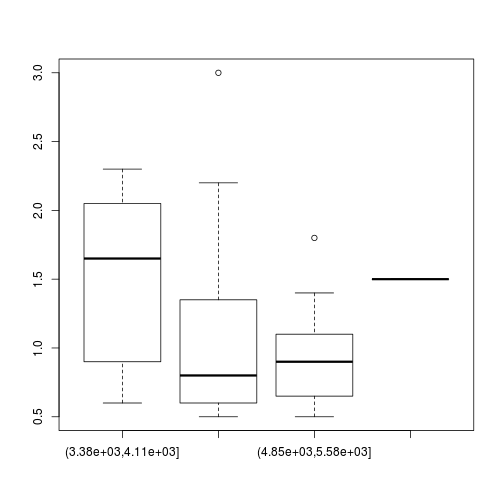
\includegraphics{figure/unnamed-chunk-15.png}
\caption{Ejemplo de boxplot}
\end{figure}

\subsubsection{1.g Exportar}

Script: ``exportar.R''

Finalmente se deberá exportar la data.frame \texttt{usaNorm} a un
archivo de texto plano. Dicho archivo se llamará ``usa-norm.csv'' y
deberá cumplir con las siguientes condiciones:

\begin{enumerate}[1.]
\item
  Deberá guardar correctamente los nombres de las filas y columnas.
\item
  El separador de columnas deberá ser el caracter ``;''.
\item
  El punto decimal debe estar indicado con el caracter ``,''
\end{enumerate}
Consulte las lecciones o la ayuda de R en \texttt{?write.table} para
determinar el comando adecuado para realizar esta operación.

\end{document}
